Once a valid path is obtained through path planning, it has to be executed by a \acs{uav}. The path is an array of coordinates. Once the \acs{uav} has reached a coordinate, it receives the next coordinate in the array until the goal is reached. The \acs{uav} reaches a coordinate when its current position is within a certain distance of the coordinate. This value is calculated with the euclidean distance.

The optimize the path, only the coordinates that go to a new direction in any axis are kept. If for example a sequence of coordinates have the same increment in x values and have the same y and z values, the only coordinates that contain useful information are the first and the last.

In figure~\ref{fig:path} the exectuable path is visualized. The red blocks are all the coordinates that are returned from the path planning algorithm, where the yellow blocks are the only points with useful information.

\begin{figure}[!h]
  \centering
  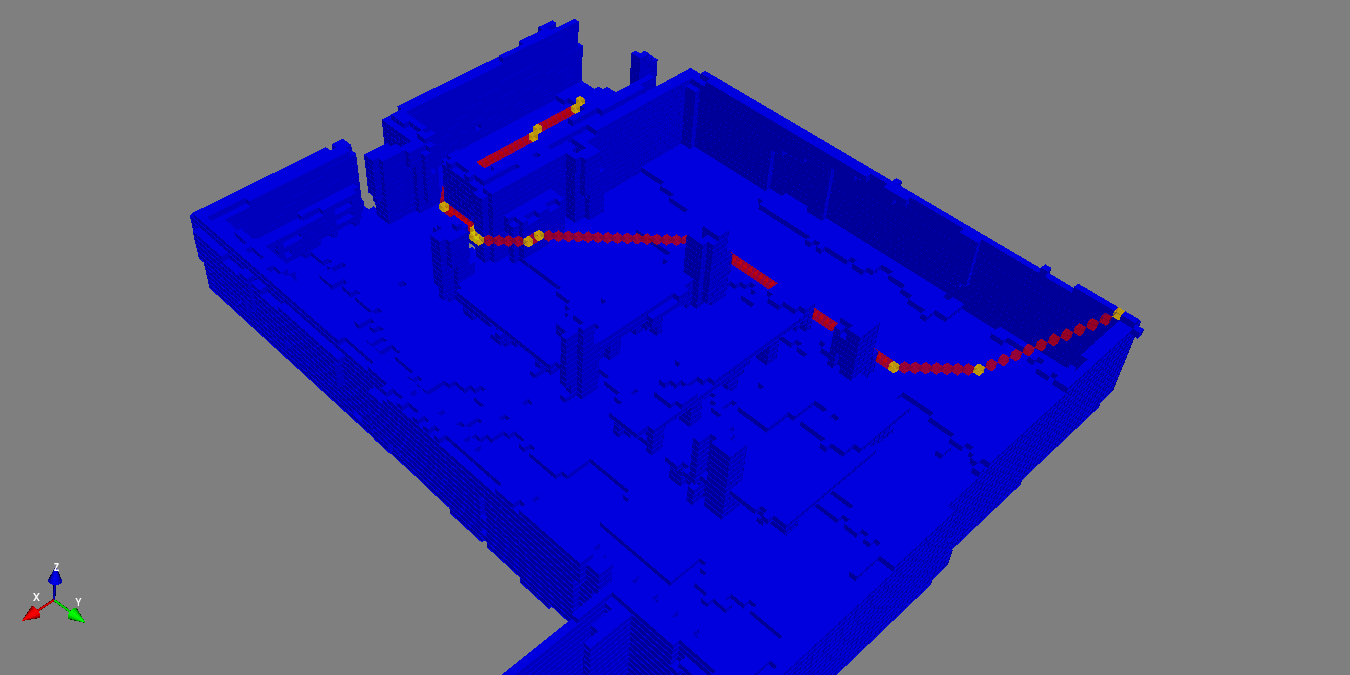
\includegraphics[width=\linewidth]{images/path.png}
  \caption{Executable path example}
  \label{fig:path}
\end{figure}